\documentclass{natureprintstyle}
%\documentclass[12pt]{nature}

\spacing{1}
\spacing{2}
\spacing{1}

%\usepackage{epsfig,caption}
\usepackage{amsmath,amssymb}
\usepackage[applemac]{inputenc}
\usepackage{graphicx}
\usepackage{color}
\usepackage{bm}
\usepackage{longtable}
\usepackage{amssymb}
\usepackage{rotating}
\usepackage{hyperref}
%\captionsetup[figure]{labelformat=empty}
%\captionsetup[table]{labelformat=empty}

\newcommand{\gt}{$>$}
\newcommand{\diamonds}{\textsc{D\large{iamonds}}}
\usepackage{hyperref}

\let\citep\cite
\let\citet\cite


\bibliographystyle{naturemag}

\title{%\sffamily 
Dynamical dark energy constraints via clustering shells of SDSS-III BOSS galaxies}
\title{%\sffamily 
Constraints on the cosmic expansion history using the small scale clustering of SDSS-III BOSS galaxies}

\author{%\sffamily 
Xiao-Dong Li,$^{1}$
Cristiano G. Sabiu,$^{2}$
Changbom Park,$^{1}$
Yuting Wang,$^{3}$
Gong-bo Zhao,$^{3}$
Hyunbae Park,$^{2}$
Arman Shafieloo,$^{2}$
Juhan Kim,$^{4,1}$
and Sungwook E. Hong$^{2}$}

\begin{document}
\maketitle
\let\thefootnote\relax\footnote{


\begin{affiliations}
  \item School of Physics, Korea Institute for Advanced Study, 85 Heogi-ro, Dongdaemun-gu, Seoul 130-722, Korea
  \item Korea Astronomy and Space Science Institute, 776, Daedeokdae-ro, Yuseong-gu, Daejeon, 305-348, Korea
  \item National Astronomy Observatories, Chinese Academy of Science, Beijing, 100012, P.R.China
  \item Center for Advanced Computation, Korea Institute for Advanced Study, 85 Hoegi-ro, Dongdaemun-gu, Seoul 130-722, Korea
\end{affiliations}
}

\vspace{-3.5mm}
\begin{abstract}
%\sffamily
We use the small scale anisotropic clustering signal of 1,133,326 galaxies from the Sloan Digital Sky Survey Data Release 
12, spanning the redshift range $0.15<z<0.69$ to place constraints on the expansion history of the Universe. 
Concentrating on the Chevallier-Polarski-Linder parametrization of dark energy, $w=w_0+w_a\frac{z}{1+z}$,
while improving upon earlier works \citep{Li2016}, 
we present a novel use of the Alcock-Paczynski (AP) test via the small scales clustering difference between redshift bins. 
This differential measure is shown to be a robust statistical tool that mitigates many systematic effects, 
allowing for competitive and unbiased constrains to be placed on cosmological parameters.
We find that our results, in combination with the CMB, BAO, SNIa and $H_0$ from Cepheid data yield, 
$\Omega_m = 0.301 \pm 0.008,\ w_0 = -1.042 \pm 0.067,\ w_a = -0.07 \pm 0.29$ (68.3\% CL). 
Adding our new AP measurements to the aforementioned results reduced the $w_0-w_a$ 2-$\sigma$ contour area by 50\%.
The AP method can be combined with the standard BAO method, 
greatly increasing the power of ongoing and future galaxy surveys in probing dark energy.
\end{abstract}

%\sffamily
%{\it Introduction.}---
The  origin  of  the late-time accelerating  expansion  of  the  universe  is  one of  the  most  salient  questions  in  contemporary cosmology. Theoretical explanations for this phenomena are many and range from a non-zero  vacuum energy and evolving  scalar  fields  remnant  from  the  big  bang, to modifications of Einstein's General Relativity\cite{2012IJMPD..2130002Y}. 
Considering the wealth of theoretical explanations, it is crucial to obtain precise and unbiased measurements of the expansion history of the Universe allowing us to 
differentiate between competing models. 

In recent years the Alcock-Paczynski (AP) test \citep{AP1979} applied to galaxy redshift samples \citep{Outram2004,Blake2011,Alam2016}, 
has allowed tight constraints to be placed on the background averaged distance scales, $D_A(z)$ and $H^{-1}(z)$.  
Assuming an incorrect cosmological model for the coordinate transformation between redshift space and comoving space, produces residual geometric distortions in the resultant galaxy distribution. 
These distortions are induced by the fact that measured distances along 
and perpendicular to the line of sight are fundamentally different. 
Measuring the ratio of galaxy clustering in the radial and transverse directions provides a probe of this AP effect.

%The BAO standard ruler method for obtaining estimates of $D_A(z)$ and $H^{-1}(z)$ is widely used and accepted by the community.
%However, since these measurements are made on large scales (~$120$Mpc), 
%they require large comoving volumes and wide redshift bins to reduce cosmic variance. 
%This results in estimates of the cosmic observables at fewer redshifts and with access to fewer Fourier modes. 
%This reduction of information hinders our attempts to test dark energy models. 

The main caveat in applying the AP test is due to the fact that 
the radial distances of galaxies are inferred from observed redshifts.
Thus AP tests are inevitably affected by peculiar the motions of galaxies,
which leads to apparent anisotropy in the clustering signal, even if the adopted cosmology is correct.
The effect, known as redshift-space distortions (RSD),
is notoriously difficult to model accurately in the statistics of galaxy clustering \citep{Ballinger1996}.

The symmetry properties of galaxy pairs\cite{Marinoni2010}  could also be used to probe the AP effect;
however, since the peculiar velocity distorts the redshifts and changes the apparent tilt angles of galaxy pairs,
this method is also seriously limited by RSD \citep{Jennings2011}.

In an effort to minimise RSD contamination, the shape of void regions\cite{Ryden1995,LavausWandelt1995}  has been 
proposed as an AP probe. This approach has the advantage that the void regions are easier to model compared with dense regions, but has limitations in that it utilizes only low density regions of the LSS and requires large samples to achieve competitive constraints \citep{Qingqing2016}.

%In an effort to overcome the RSD problem, 
%\citep{Li2016} proposed to apply the AP effect to clustering on small scales. 
%However, redshift space distortions affect the angular clustering of galaxies, mimicking a signal similar to the AP effect, 
%thus contaminating the cosmological information.

Previously, we proposed to use the  {\it redshift dependence} of the AP distortion\cite{Li2014} as a way of mitigating the RSD effect. The clustering anisotropies produced by RSD are, although large, close to uniform in magnitude over a wide range in redshift.  However, if cosmological parameters are incorrectly chosen resulting in an AP effect, 
the anisotropy in the clustering signal has a clear redshift dependence
(as an illustration, Fig.\ref{fig_xy} shows how the shape distortion of objects varies with distance (i.e., redshift) 
when incorrect cosmologies are used to infer distances).
In a later work\cite{Li2015}, we developed an AP methodology 
that utilises the redshift dependence of the galaxy 2-point correlation function (2pCF), 
measured as a function of angle between the galaxy pair and line-of-sight (LoS).


In an earlier work\citep{Li2016} we applied this AP method to galaxies from the 3rd incarnation of the Sloan Digital Sky Survey (SDSS-III). 
Combining the method with measurements of the Cosmic Microwave Background (CMB), type Ia supernovae (SNIa), 
baryon acoustic oscillations (BAO), and $H_0$,
we obtained very tight constraints of $ \Omega_m = 0.301 \pm 0.006,\ w=-1.054 \pm 0.025$.
In reducing the RSD effect, 
we were able to use galaxy clustering on scales down to 6 $h^{-1}$Mpc,
which is a major advance in extracting cosmological information 
on small scales where galaxy clustering is strong and there are many independent structures.

In this paper, we continue to develop our previous methodology and proceed to infer the constraints on dynamical dark energy. 
We will present a slightly improved methodology to that of our previous work\citep{Li2016}, 
allowing for faster likelihood estimation and thus the exploration of larger, higher dimensional parameter spaces
(see Methods for details). 
The methodology we will present here, can be applied to any model of dynamical dark energy, 
or indeed any appropriately chosen parametric or non-parametric decomposition of the cosmic expansion history. 
However, as a first step, in this paper we will focus on the widely used Chevallier-Polarski-Linder (CPL) parametrization\cite{CPL_CP,CPL_L},
\begin{equation}
w(z) = w_0 + w_a (1-a) = w_0 + w_a \frac{z}{1+z}.
\end{equation}
This parametrization characterizes dark energy equation-of-state (EoS) by two free parameters.
$w_0$ determines the present-day value, while parameter $w_a$ characterizes the first-order derivative of $w$ with respect to $a$. 
The CPL parametrization has many obvious advantages, for instance, a manageable parameter space, 
the bounded behavior at high redshift, 
and the ability to accurately reconstruct many dark energy theories\cite{CPL_L}. 
So it was widely used in the literature to reconstruct dark energy from observations.


%The CPL parametrization has been widely used to study the dynamical properties of dark energy in literature.
The Planck team has released the {\texttt {COSMOMC}} \citep{LB2002} outputs of four MCMC ``chains'' in the CPL model, 
using a combination of four datasets:
the full-mission Planck observations of CMB temperature and polarization anisotropies \cite{Planck2015},
the BAO distance priors measured from SDSS DR11 \citep{Anderson2013}, 6dFGS \citep{6dFGS} and SDSS MGS \citep{MGS},
the ``JLA'' SNIa sample \citep{JLA},
and the Hubble Space Telescope measurement of $H_0=70.6\pm3.3$ \cite{Riess2011,E14H0}.
These MCMC chains contain the CMB+BAO+SNIa+$H_0$ likelihood computed for $\sim$37,000 sets of cosmological parameters,
yielding constraints of %$ \Omega_m = 0.309 \pm 0.010, w_0 = -0.938 \pm 0.109, w_a = -0.38 \pm 0.41$.
\begin{equation}
 \Omega_m = 0.309 \pm 0.010, w_0 = -0.938 \pm 0.109, w_a = -0.38 \pm 0.41.
\end{equation}

To derive the constraints combined with our AP method,
we then compute the likelihood of the SDSS LOWZ+CMASS AP measurements for each of the parameter combinations provided in the Planck chain. 
To do this, we splited the 1,133,326 galaxies from the SDSS DR12 into six redshift bins,
measured the 2pCF (on scales of 6-40 $h^{-1}$Mpc) in these redshift bins (see Fig.\ref{fig_nbar}).
This enables us investigating the redshift evolution of anisotropic clustering.
We subtracted the systematic effects based on estimations from mocks made from Horizon Run 4 simulations \citep{HR4},
and used a $\chi^2$ function to assess the redshift dependence.
(see Methods for further explanations).

After adding the log-likelihoods of the Planck team sample with ours, 
while also multiply the sample weights by our likelihoods, 
we derive the CMB+BAO+SNIa+$H_0$+AP constraints on CPL parameters, %$\Omega_m = 0.301 \pm 0.008, w_0 = -1.042 \pm 0.067, w_a = -0.07 \pm 0.29$.
\begin{equation}
\Omega_m = 0.301 \pm 0.008, w_0 = -1.042 \pm 0.067, w_a = -0.07 \pm 0.29.
\end{equation}
While the central values of parameters do not shift appreciably,
the error bars of $w_0$ and $w_a$ are reduced by 38.4\% and 29.7\%, respectively.% $$-40\%$ by adding our method into the analysis.

The marginalised constraints on $w_0-w_a$ are shown in the left panel of Fig.\ref{fig_con}.
Adding our new AP constraints significantly reduces the allowable parameter space. 
This can also be visualise as allowable bands in $w(z)$ as can be seen in the right panel of Fig.\ref{fig_con}.  

The derived cosmological constraints are fully consistent with a cosmological constant dark energy component having no evolution.
Adding the new AP method to the CMB+BAO+SNIa+$H_0$ constraints reduces the statistical errors on many parameters by $\sim$30-40\% 
and reduces the $w_0-w_a$ (95.4\% CL) contour by 50\%.
This reveals the constraining power of the small scale AP effect for probing the redshift evolution of dark energy.

We performed a thorough test of all the possible variables in our methodology.
Figure \ref{fig_contest} shows that 
the result is unaffected by the line-of-sight $\mu$-cut, 
the number of angular bins, 
the range of radial integration and the choice of fiducial cosmology. 
%we adopt $\mu_{\rm max}=0.99\ (0.85)$ to include more (less) regions near the LOS,
%decrease the number of angular bins to $n_{\mu}=15-20$,
%change the range of clustering to $8-30 \rm Mpc/h$,
%change the fiducial cosmology to $\Omega_m=0.26,\ w=-0.6$,
%exclude 1 or 2 high redshift bins,
%or reduce the number of mocks to 1000.
The most striking point to note in our testing is that the 
shift in contour position is very small even when we do not include the systematic correction.
This is reassuring, since we may have worried that {\it cosmological dependence} 
of the systematic correction could influence the final result. 

In summary, we previously proposed to constrain cosmological parameters via 
the redshift dependence of anisotropic galaxy clustering\cite{Li2016}.
This approach enables a robust AP test on relatively small scales.
In this paper we improved the methodology and obtained tight constraints on the CPL parametrization of dark energy.
%using 1,133,326 galaxies from the Sloan Digital Sky Survey Data Release 
%12 spanning the redshift range $0.15<z<0.69$ . 
%Adding our constraints to the CMB+SNIa+BAO+$H_0$ combination, the $w_0-w_a$ contour was reduced by $\sim50$\%.
The AP method presented in this work has many advantages over the `traditional' galaxy clustering method.
Since it works with the redshift evolution of the anisotropic clustering signal it significantly reduces the effect of systematics. 
It avoids the great difficulty in accurate modelling of the RSD, non-linear clustering and galaxy bias.
It is applicable on much smaller scales, allowing for the inclusion of more $k$-modes and hence more information. 

The presented method of clustering shells can be applied to many spectroscopic galaxy surveys. 
The method is complimentary to the BAO method and the two methods can be combined together, 
increasing (by roughly twice) the power of ongoing and future surveys, with little to no additional cost.
We expect this approach will play an important role in helping us unveiling the mystery of dark energy.


\begin{thebibliography}{10}
\expandafter\ifx\csname url\endcsname\relax
  \def\url#1{\texttt{#1}}\fi
\expandafter\ifx\csname urlprefix\endcsname\relax\def\urlprefix{URL }\fi
\providecommand{\bibinfo}[2]{#2}
\providecommand{\eprint}[2][]{\url{#2}}

\bibitem{Li2016}%[Li et al.(2016)]
Li, X.-D., Park, C., \& Sabiu, C.G., et al. 2016, ApJ, 832, 103

\bibitem{2012IJMPD..2130002Y}%[Yoo \& Watanabe(2012)]
Yoo, J., \& Watanabe, Y.\ 2012, International Journal of Modern Physics D, 21, 1230002 

\bibitem{AP1979}%[Alcock \& Paczynski(1979)]
Alcock, C., \& Paczynski, B. 1979, Nature, 281, 358  

\bibitem{Outram2004}%[Outram et al.(2004)]
Outram, P.J., Shanks, T., Boyle, B.J., Croom, S.M., Hoyle, F., Loaring, N.S., 
Miller, L., \& Smith, R.J. 2004, MNRAS, 348, 745  

\bibitem{Blake2011}%[Blake et al.(2011)]
Blake, C., Glazebrook, K., \& Davis, T. M., 2011, MNRAS, 418, 1725  

\bibitem{Alam2016}%[Alam et al.(2016)]
Alam, S., Ata, M., \& Bailey, S., et al. 2016,
submitted to MNRAS (arXiv:1607.03155)

\bibitem{Ballinger1996}%[Ballinger, Peacock \& Heavens 1996]
Ballinger, W.E., Peacock, J.A., \& Heavens, A.F. 1996, MNRAS, 282, 877  

\bibitem{Marinoni2010}%[Marinoni \& Buzzi(2010)]
Marinoni, C., \& Buzzi, A. 2010, Nature, 468, 539  

\bibitem{Jennings2011}%[Jennings et al.(2011)]
Jennings, E., Baugh, C.M., \& Pascoli, S. 2011, MNRAS, 420, 1079  

\bibitem{Ryden1995}%[Ryden(1995)]
Ryden, B.S. 1995, ApJ, 452, 25  

\bibitem{LavausWandelt1995}%[Lavaux \& Wandelt(2012)]
Lavaux, G., \& Wandelt, B.D. 2012, ApJ, 754, 109  

\bibitem{Qingqing2016}%[Mao et al. (2016)]
Mao, Q., Berlind, A.A., Scherrer, R.J., et al. 2016, submitted to ApJ


\bibitem{Li2014}%[Li et al.(2014)]
Li, X.-D., Park, C., Forero-Romero, J., \& Kim, J. 2014, ApJ, 796, 137

\bibitem{Li2015}%[Li et al.(2015)]
Li, X.-D., Park, C., Sabiu, C.G., \& Kim, J. 2015, MNRAS, 450, 807 

\bibitem{CPL_CP}
Chevallier, M, \& Polarski, D. 2001, Int. J. Mod. Phys. D,  10, 213

\bibitem{CPL_L}
Linder, E. V. 2003, Phys. Rev. Lett, 90, 091301

\bibitem{LB2002}%[Lewis \& Bridle (2002)]
Lewis, A., \& Bridle, S. 2002, Phys. Rev. D, 66, 103511

\bibitem{Planck2015}%[Ade et al. (2015)]
Ade, P.A.R., Aghanim, N., \& Arnaud, M., et al. 2016, A\&A, 594, A13 

\bibitem{Anderson2013}%[Anderson et al.(2013)]
Anderson, L., Aubourg, \'E., \& Bailey, S. et al. 2014, MNRAS, 441, 24 

\bibitem{6dFGS}%[Beutler et al.(2011)]
Beutler, F., Blake, C., \& Colless, M., et al. 2011, MNRAS, 416, 3017

\bibitem{MGS}%[Ross et al.(2015)]
Ross, A.J., Samushia, L., \& Howlett, C., et al. 2015, MNRAS, 449, 835

\bibitem{JLA}%[Betoule et al.(2014)]
Betoule, M., Kessler, R., \& Guy, J., et al. 2014, A\&A, 568, 32

\bibitem{Riess2011}%[Riess et al.(2011)]
Riess, A.G., Macri, L., \& Casertano, S., et al. 2011, ApJ, 730, 119

\bibitem{E14H0}%[Efstathiou (2014)]
Efstathiou, G. 2014, MNRAS, 440, 1138

\bibitem{HR4}%[Kim et al.(2015)]
Kim, J., Park, C., L'Huillier, B., \& Hong, S. E. 2015, JKAS, 48, 213

%\bibitem{Lee12}
%\bibinfo{author}{Lee}, E.~J., {Murray}, N., {Rahman}, M. 
%\newblock \bibinfo{title}{Milky Way Star-forming Complexes and the Turbulent Motion of the Galaxy's Molecular Gas.}
%\newblock{\it Astrophys. \ J.}{\bf\, 752}, 146-159 (2012).



%%%% For methods
\bibitem{Reidetal:2016}%[Reid et al.(2016)]
Reid, B., Ho, S., \& Padmanabhan, N., et al.  2016, MNRAS, 455, 1553

\bibitem{komatsu2011}%[Komatsu et al.(2011)]
Komatsu, E., Smith, K. M., \& Dunkley, J., et al. 2011, ApJS, 192, 18  

\bibitem{hong2016}%[Hong et al.(2016)]
Hong, S.E., Park, C.,\&  Kim, J. 2016, ApJ, 823, 103

\bibitem{MDPATCHY}%[Kitaura et al.(2015)]
Kitaura, F.S., Rodriguez-Torres, S., Chuang, C.-H., et al.2016, MNRAS, 456, 4156

\bibitem{Hartlap}%[Hartlap et al.(2006)]
Hartlap J., Simon P. \& Schneider P. [astro-ph/0608064].

\bibitem{Percival2014}%[Percival et al.(2014)]
Percival, W.J., Ross, A.J., \& S\'{a}nchez, A.G., et al. 2014, MNRAS, 439, 2531

\end{thebibliography}

\begin{addendum}
\item [Acknowledgements] 
We thank the Korea Institute for Advanced Study for providing computing resources (KIAS Center for Advanced Computation Linux Cluster System).
CGS acknowledges support from the National Research Foundation (NRF,  \#2017R1D1A1B03034900). 
We thank Stephen Appleby, Seokcheon Lee, Maurice van Putten, Graziano Rossi and Yi Wang for helpful discussions.


\item[Author contributions] 

X.L. computed the approximated 2pCFs in the many cosmologies, did the statistical analysis and computed the likelihoods, 
derived the final cosmological constraints, and conducted the robustness tests. 
C.S. wrote the code for computing the 2pCFs, and contributed in the likelihood methodology and the robustness tests. 
C.P. contributed in the concept of using the redshift dependence to do AP test.
He also contributed in the statistical methods of LSS, the likelihood methodology,
the horizon run simulations, the systematic corrections, and the robustness tests.
Y.W. and G.Z. contributed in the computing of approximated 2pCFs in non-fiducial cosmologies and the robustness tests.
H.P. contributed in the 2pCF measurements, the likelihood computation, and the systematic correction.
A.S. contributed in the fast computation of likelihoods in non-fiducial cosmologies, and the cosmological interpretation of the results.
J.K. and S.H. performed the Horizon Run 4 simulations and created the mock galaxy samples.
All authors commented on the manuscript.


\item[Author information]
%Supplementary information is available for this paper. 
Reprints and permissions information is available at \href{www.nature.com/reprints}{www.nature.com/reprints}.
Correspondence and requests for materials should be addressed to X.L. (e-mail: \href{mailto:xiaodongli@kias.re.kr}{xiaodongli@kias.re.kr}).

\item[Competing interests]
The authors declare no competing financial interests.

\end{addendum}



\newpage

\begin{figure}[tb]
   \centering{
   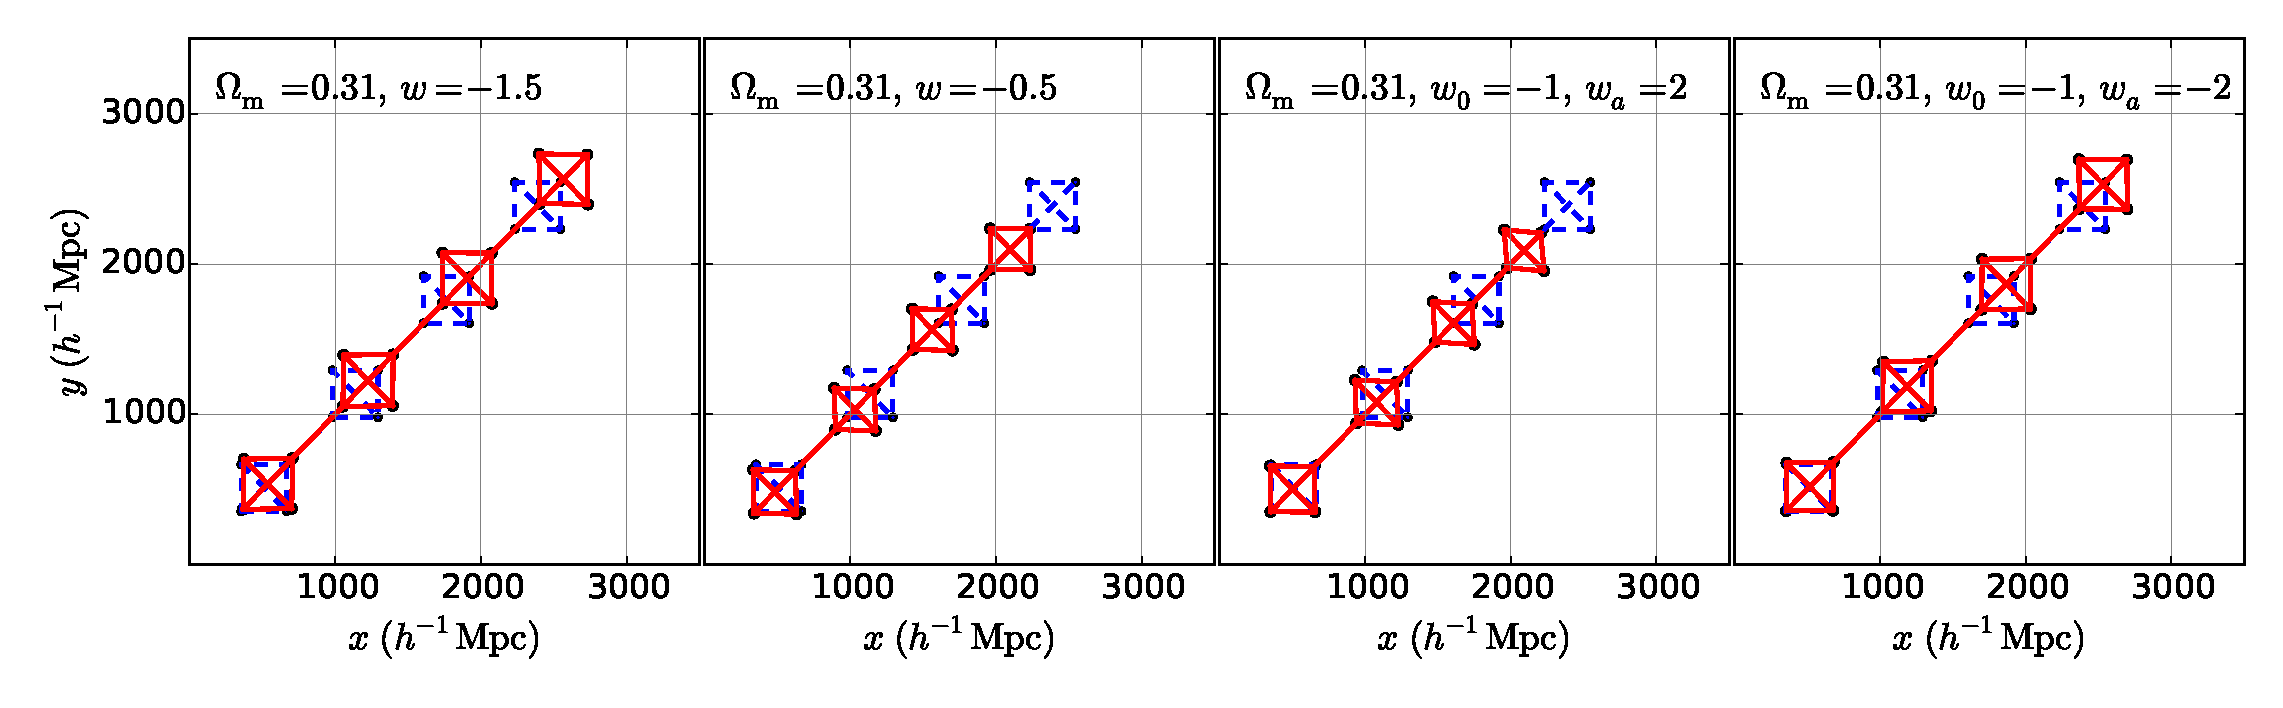
\includegraphics[height=5cm]{fig_xy.eps}
   }
   \vspace{-2mm}
   \caption{\label{fig_xy}
   {\bf The distance dependence of the shape distortion in four wrongly assumed cosmologies}.
   Assuming a true cosmology of $\Omega_m=0.31$, $w=-1$.
   There are four perfect squares with their true shapes plotted in blue dashed lines.
   They are measured by an observer located at the origin, and the distances are reprojected in the four wrong cosmologies.
   The apparently distorted shapes are plotted in red solid lines.
   }
   \vspace{-4mm}
\end{figure}

\begin{figure}[tb]
   \centering{
   %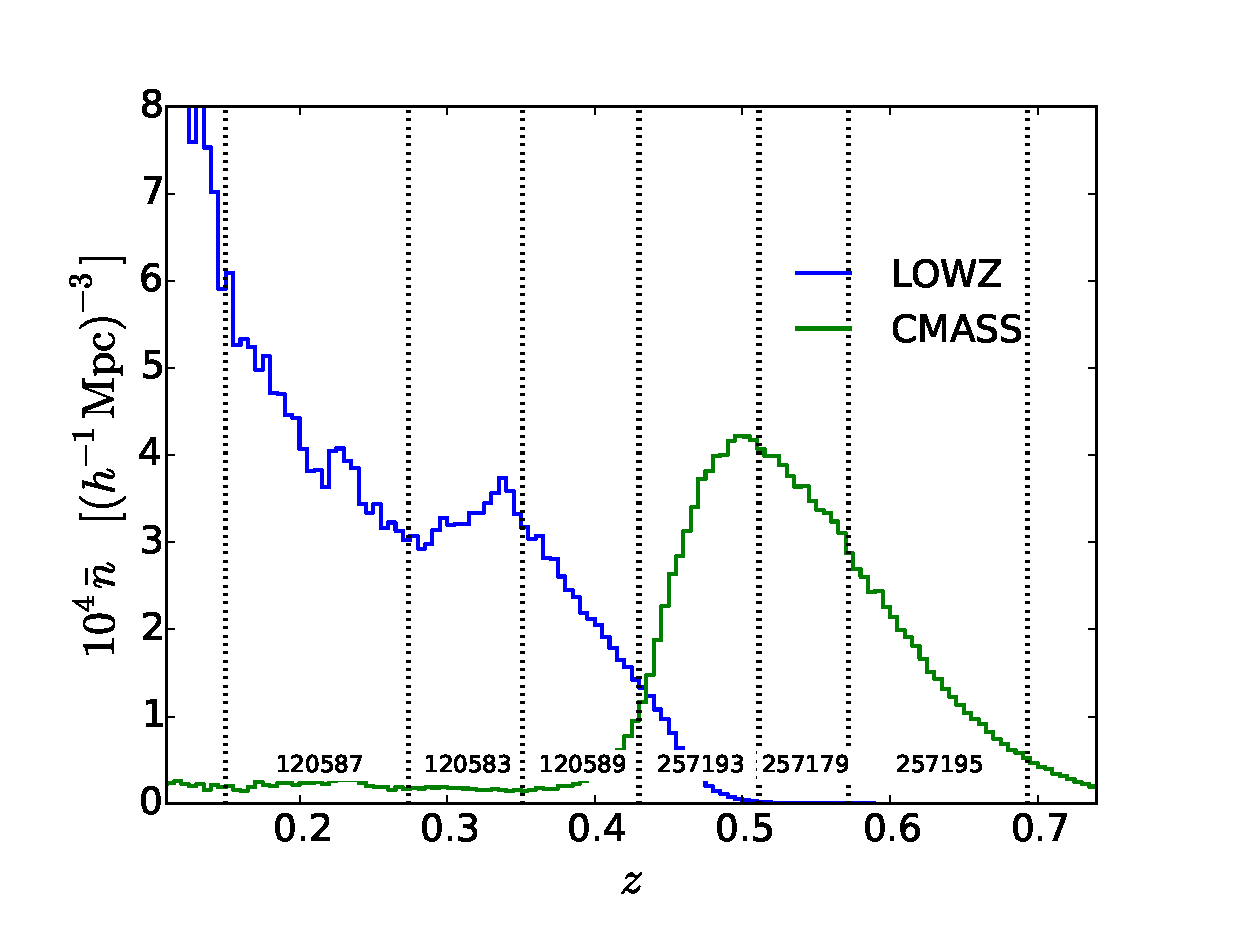
\includegraphics[height=5.3cm]{fig_nbar.eps}
   %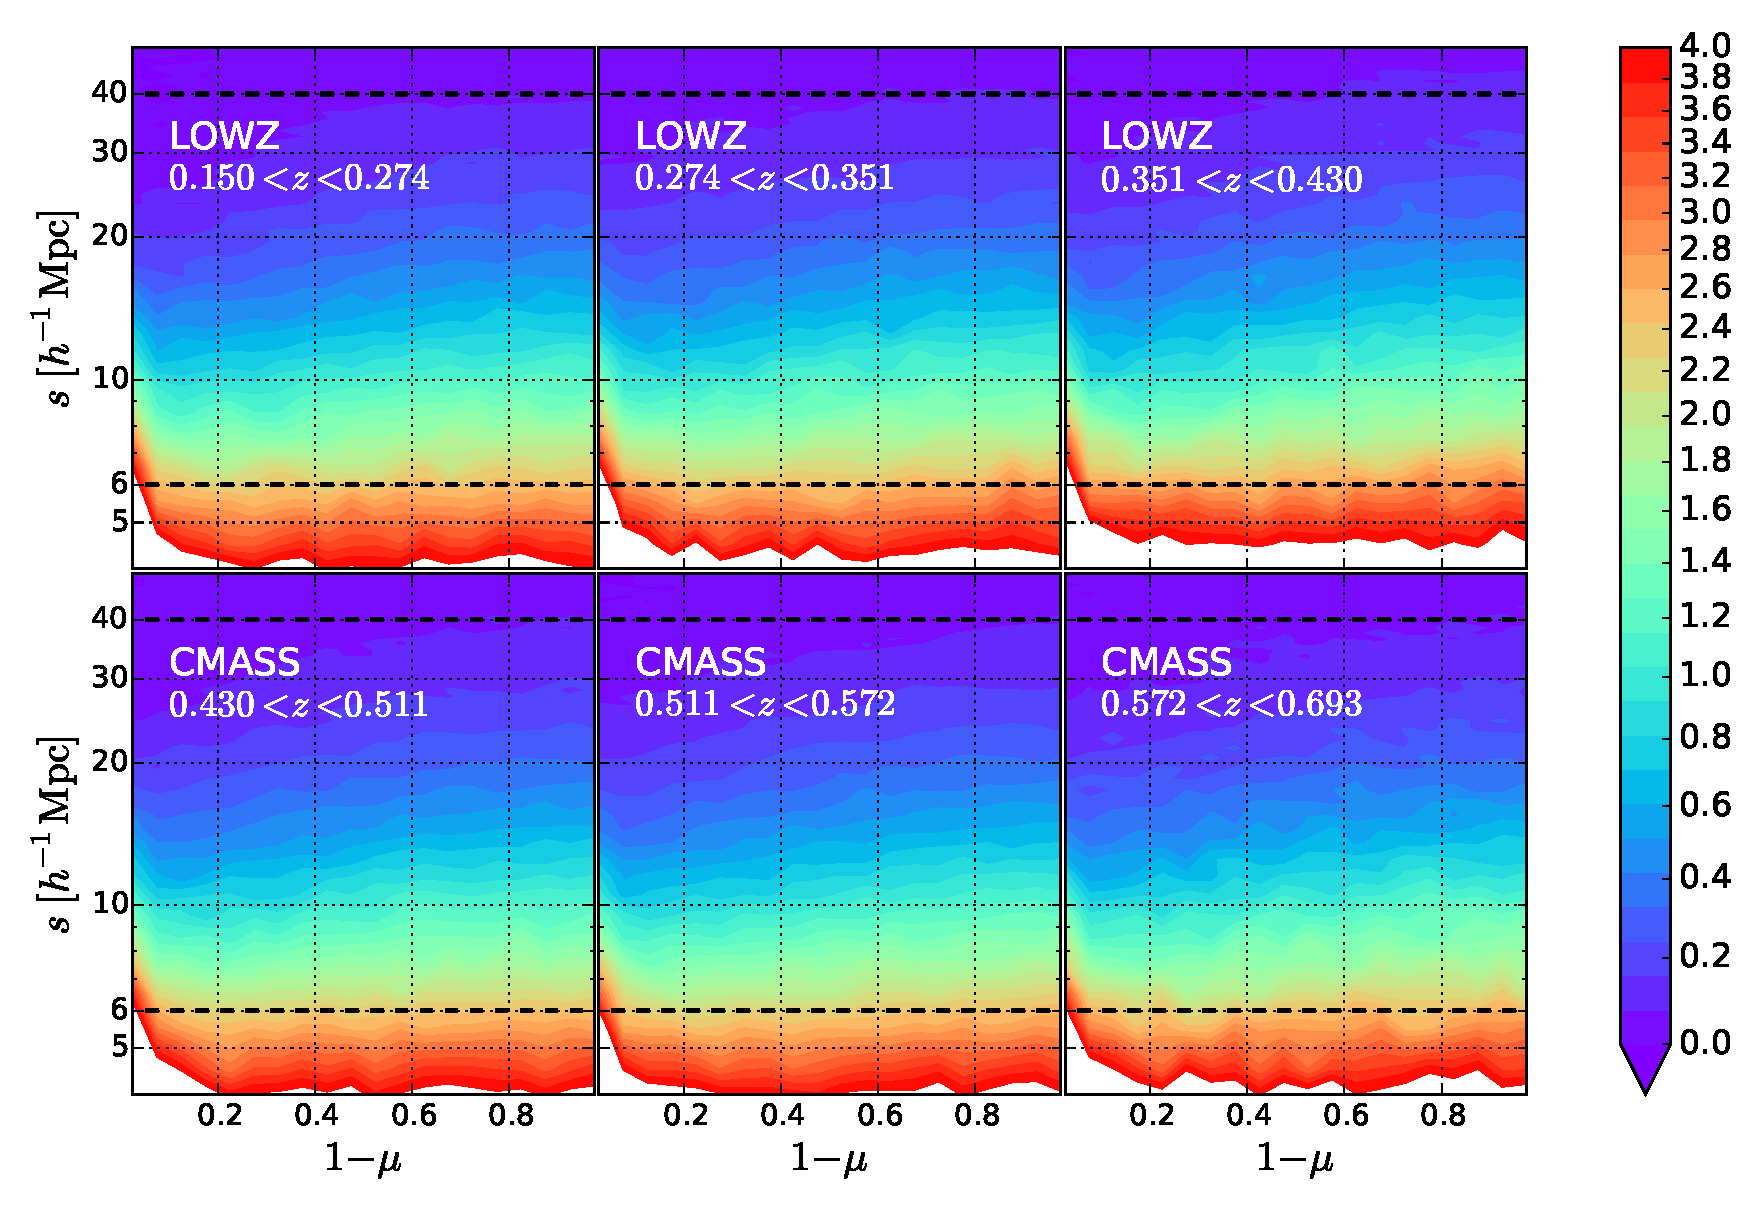
\includegraphics[width=7cm,]{fig_2pcf.eps}
   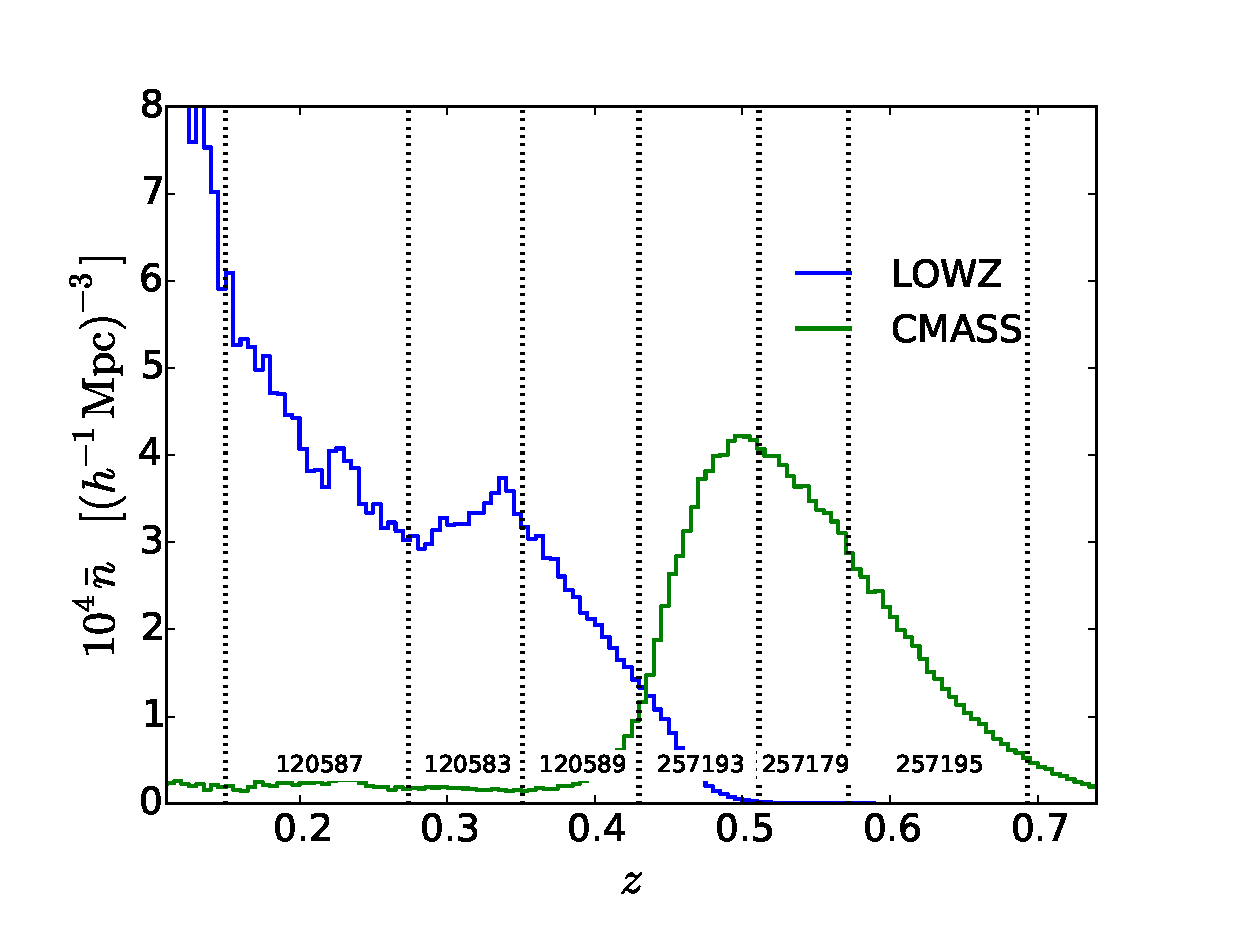
\includegraphics[width=14cm]{fig_nbar.eps}
   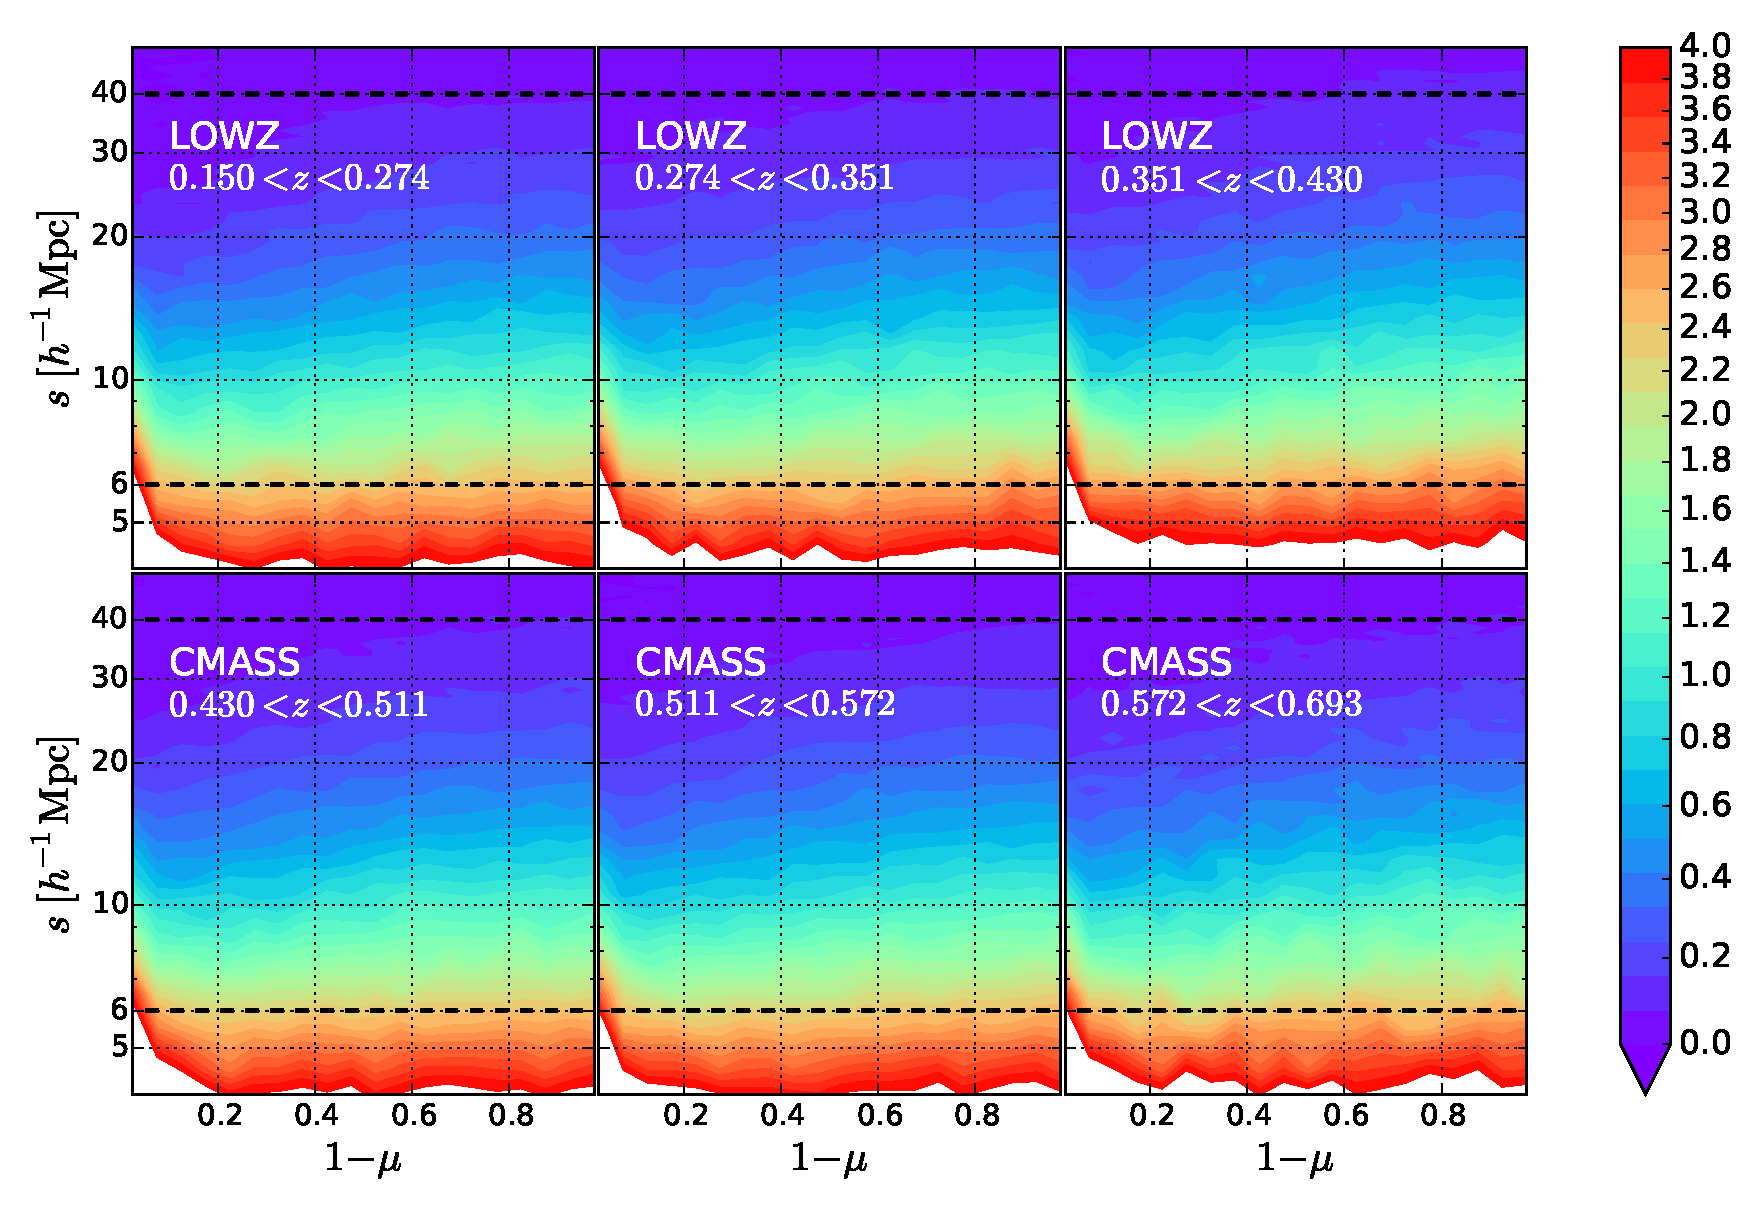
\includegraphics[width=14cm,]{fig_2pcf.eps}
   }
   \caption{\label{fig_TpCF}
   {\bf Spliting the SDSS galaxies into six redshiftbins, and measuring the correlation function.}
   Upper panel: We split the BOSS DR12 galaxies into six redshift bins to measure the evolution of shape distortion.
   The blue and green solid histograms show the redshift density distribution of LOWZ and CMASS galaxies in the $\Omega_m=0.31$ $\Lambda$CDM. 
   The vertical dashed lines define the six redshift bins that are used to cut the samples.                                       .
   The number of LOWZ/CMASS galaxies in the three low/high redshift bins are listed.
   Lower panel: 2D contour map of measured $\xi$ as a function of $\mu$ and $s$, from the six redshift bins of LOWZ and CMASS samples, 
      in the cosmology of $\Omega_m=0.31$ $\Lambda$CDM model.
    The black dashed lines mark the clustering region 6-40\ Mpc/h studied in the AP method.
    The six contour maps have rather similar appearance, implying small redshift evolution of $\xi$ from RSD.
   }
\end{figure}

\begin{figure}[tb]
   \centering{
   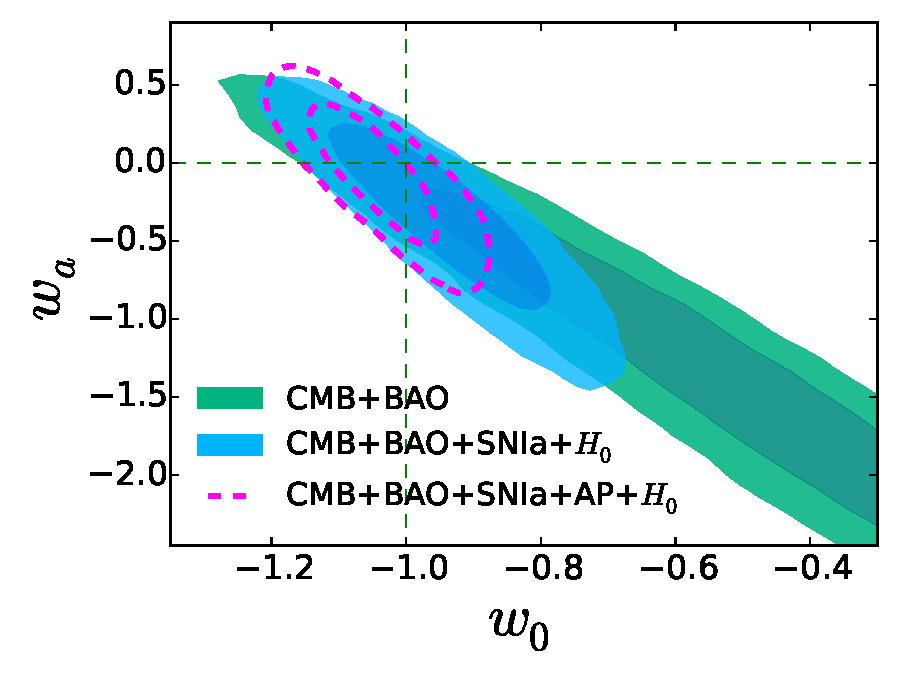
\includegraphics[height=7cm,natwidth=6,natheight=4.5]{figCPL_b.pdf}
   %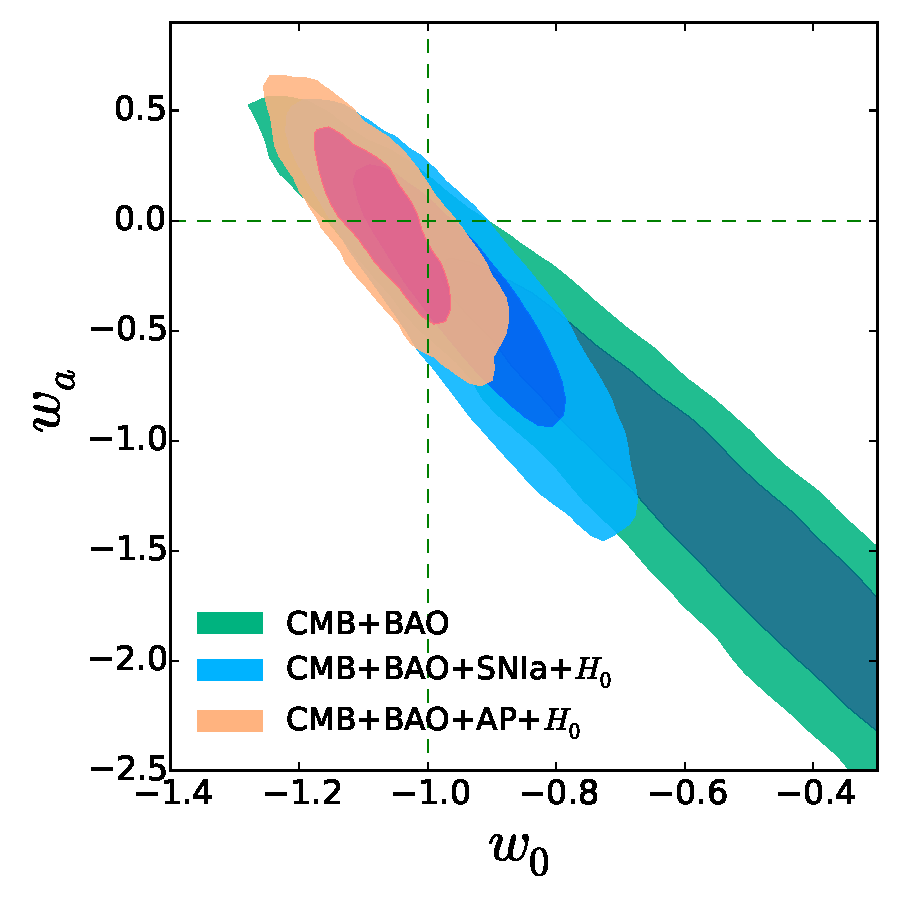
\includegraphics[width=5.5cm,natwidth=4,natheight=4]{figCPL_b_BAOSNIaAP.pdf}
   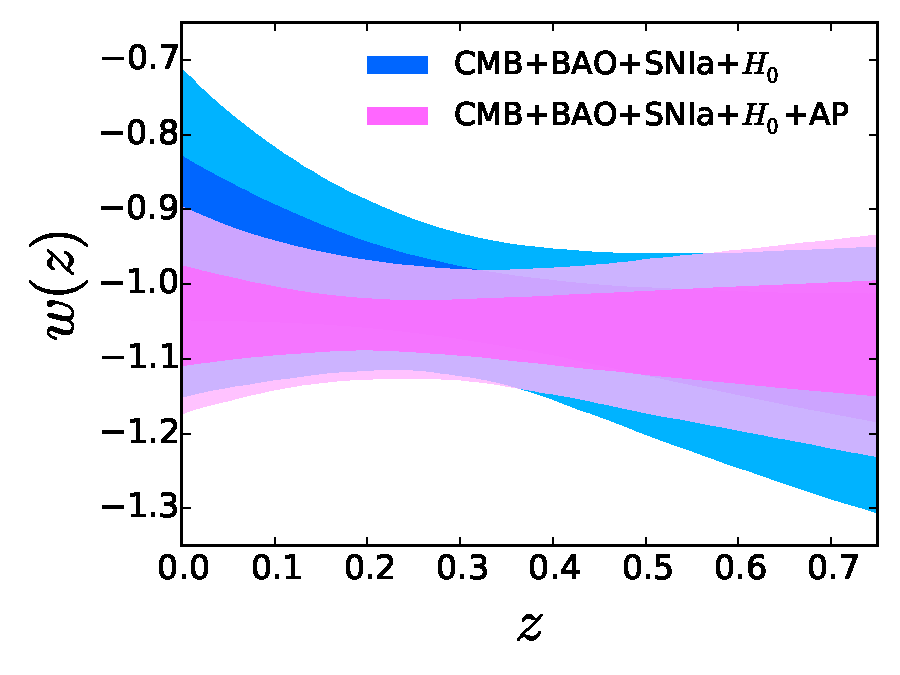
\includegraphics[height=7cm,natwidth=6,natheight=4.5]{figCPL_d.pdf}
   }
   \caption{\label{fig_con}
   {\bf Cosmological constraints on the CPL dark energy parametrization $w=w_0+w_a\frac{z}{1+z}$.}
   Upper panel: 68.3\%, 95.4\% CL likelihood contours in the  $w_0-w_a$ plane.
   %Results are consistent with $\Lambda$CDM.
   The constrained area is significantly reduced after combined with the AP method.
   %This shows the power of the AP method in constraining dynamical dark energy.
   %Middle panel: $w_0-w_a$ likelihood contours using datasets of CMB+BAO, CMB+BAO+SNIa+$H_0$ and CMB+BAO+AP+$H_0$.
   %When combined with CMB+BAO, AP method yields much tighter constraints than SNIa.
   Lower panel: Redshift evolution of $w(z)$, with/without adding the AP constraint.
   Adding AP tightens the constraints and reduces the redshift evolution of $w$ (tilt of $w(z)$).
   }
\end{figure}

\begin{figure}[tb]
   \centering{
   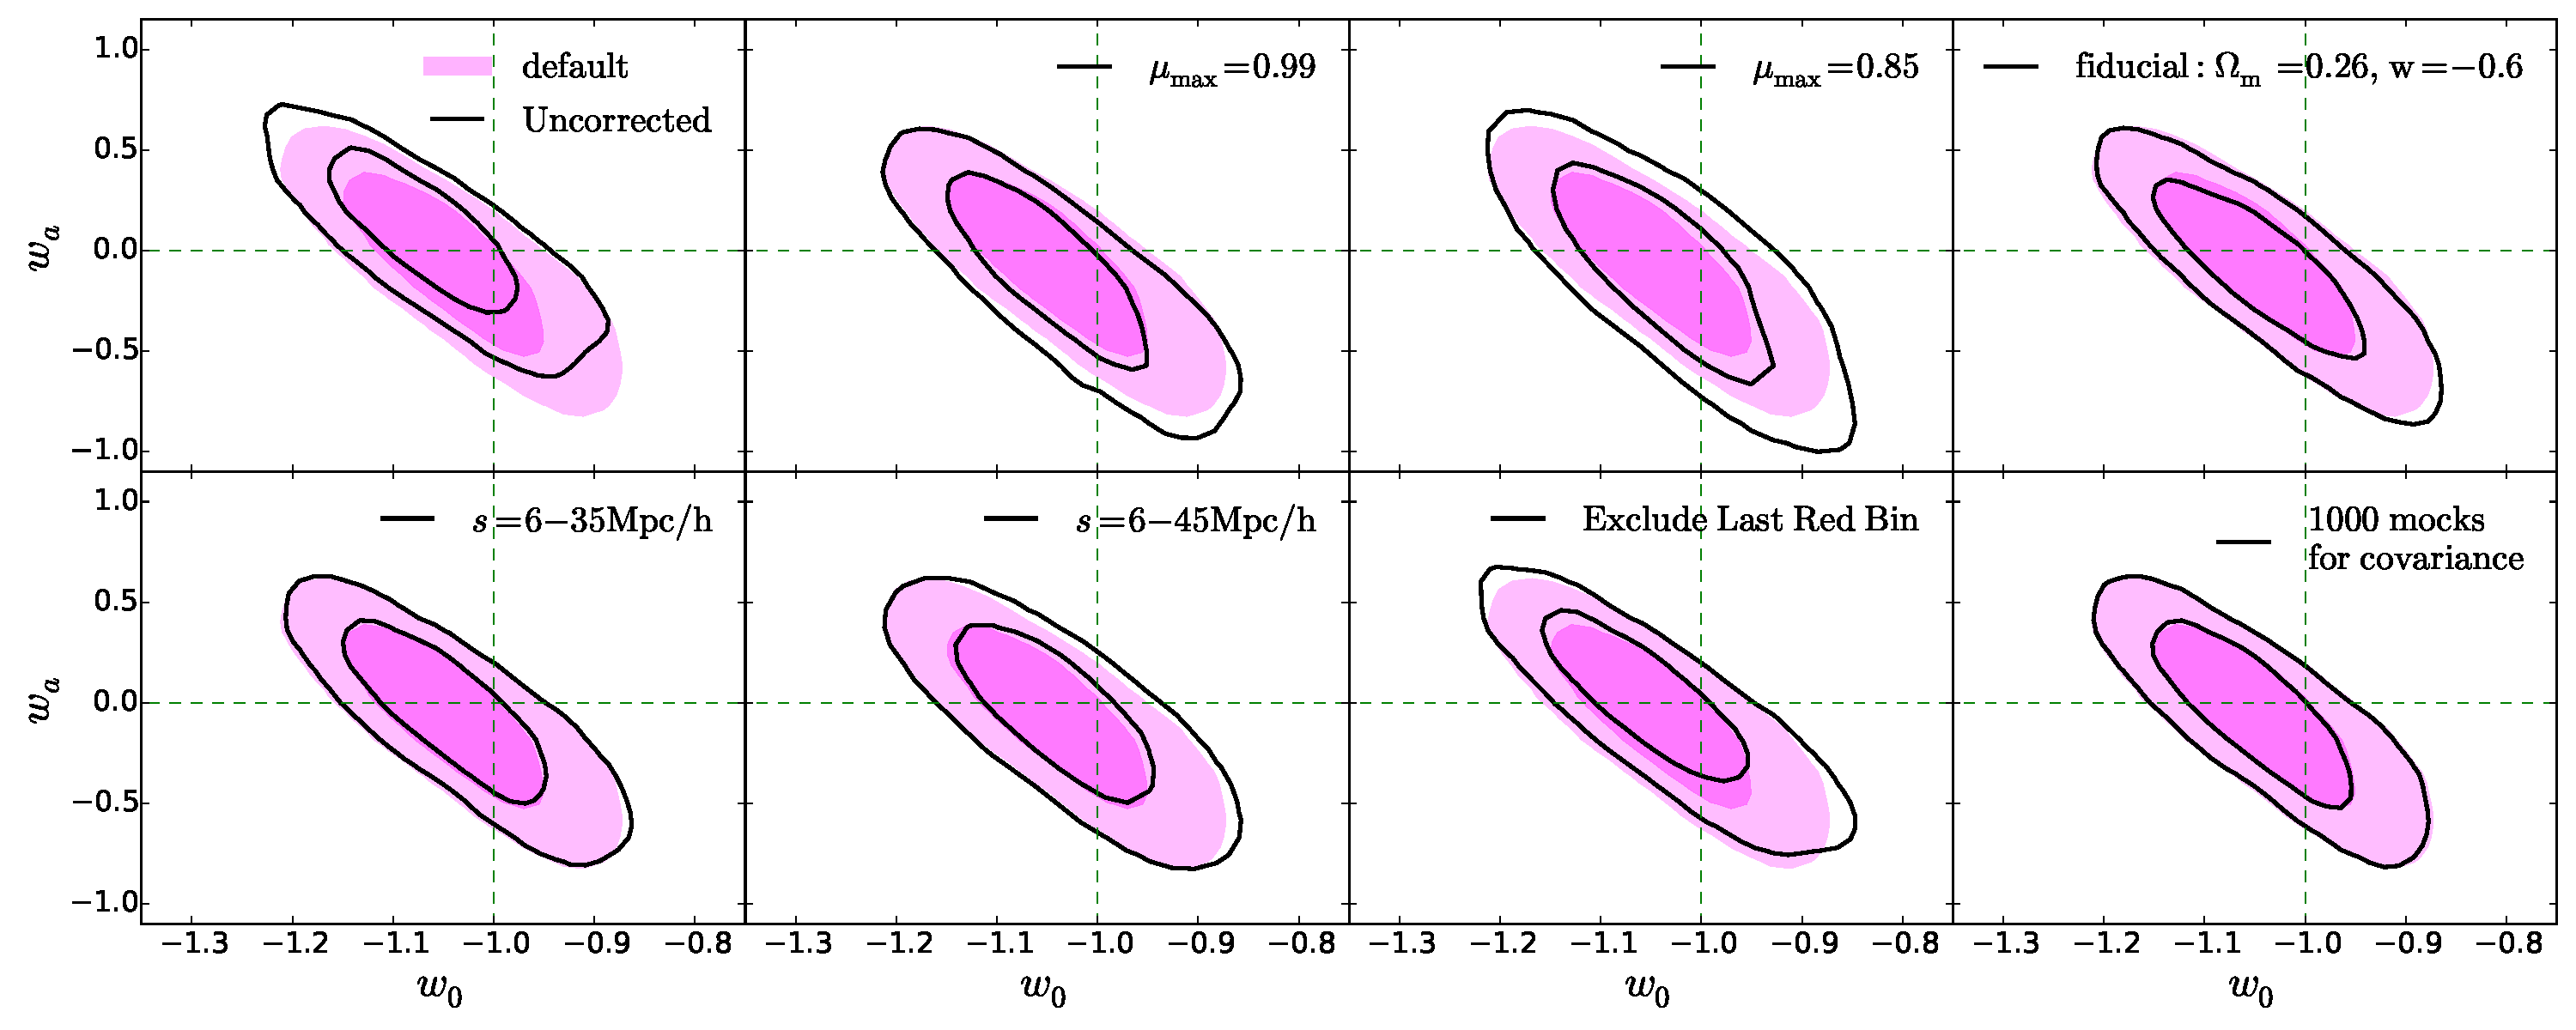
\includegraphics[width=16cm,natwidth=6,natheight=5]{fig_con_tests.pdf}
   %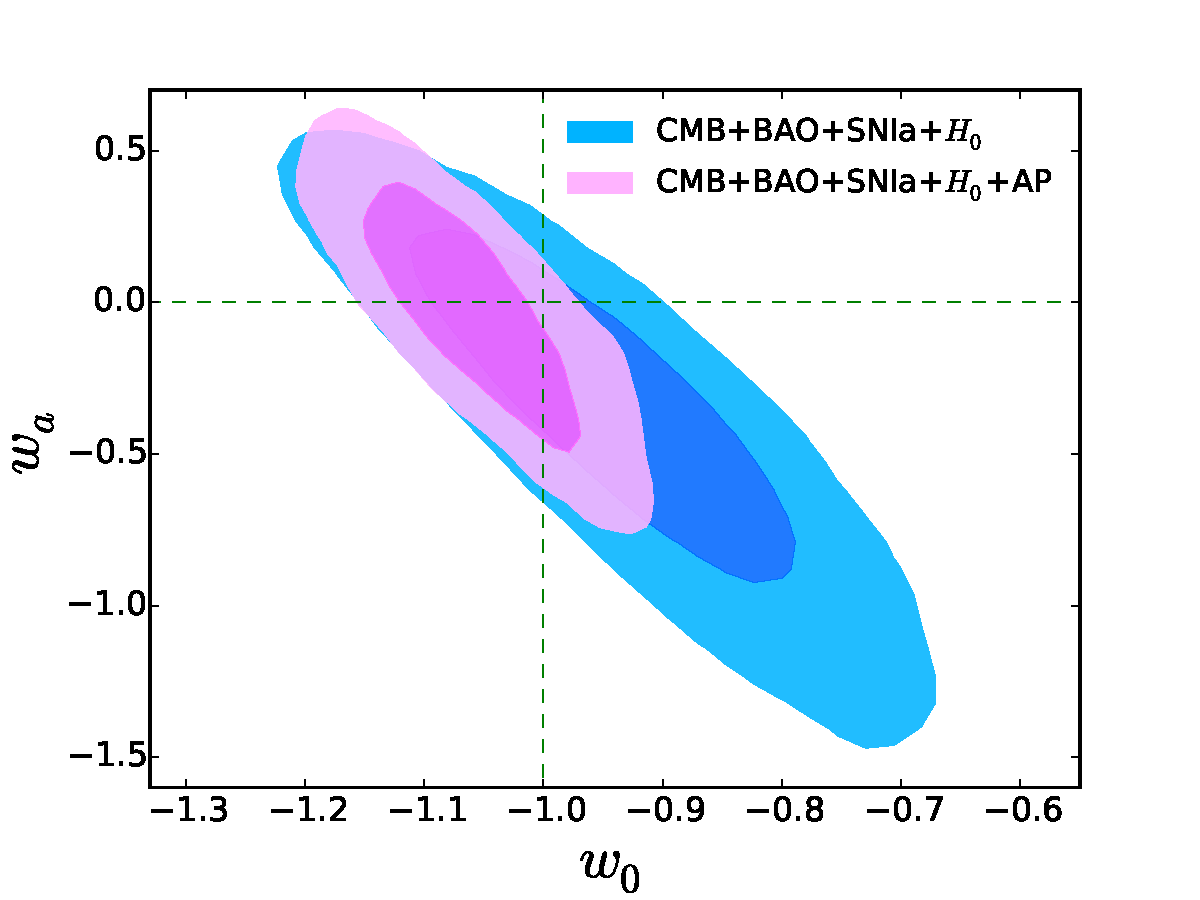
\includegraphics[width=9cm,natwidth=4,natheight=4]{fig2b.pdf}
   %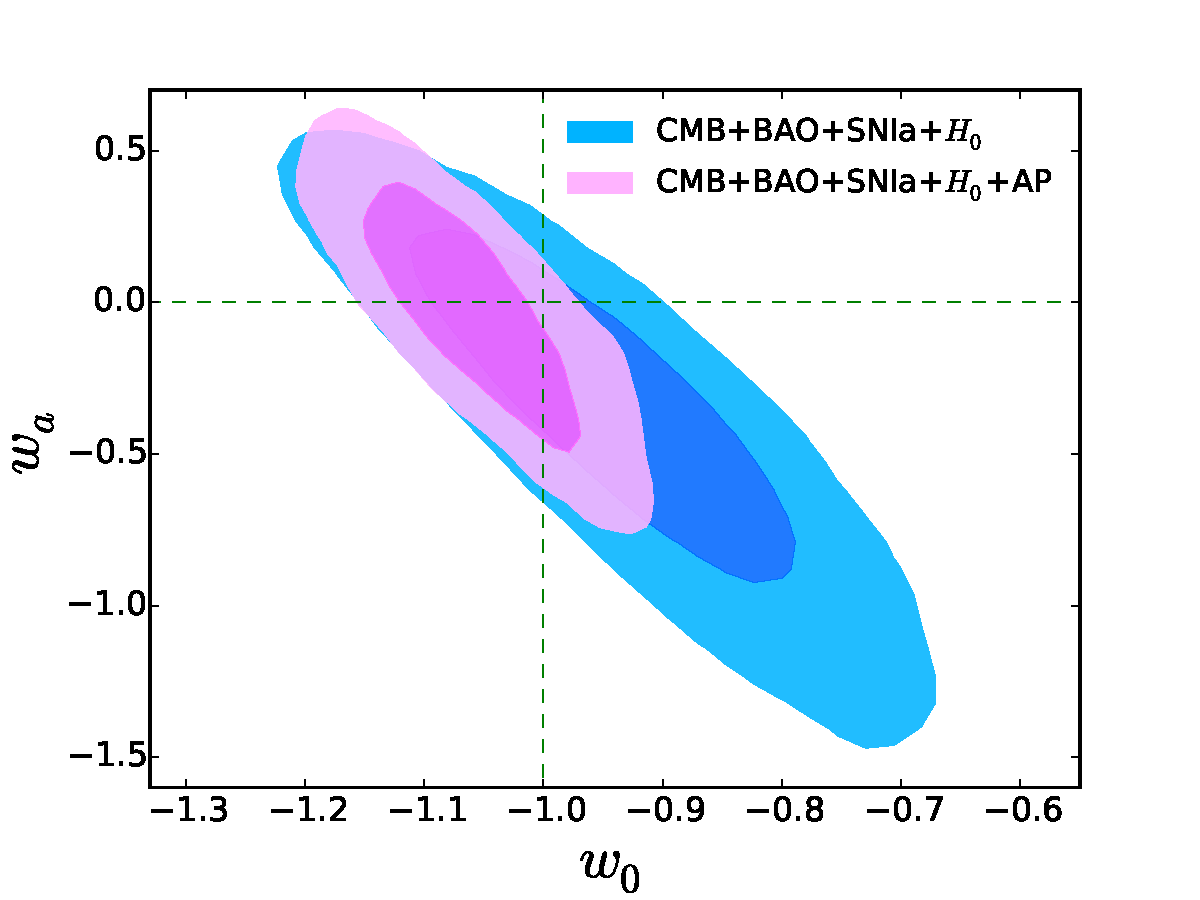
\includegraphics[height=8cm]{fig2b.pdf}
%   \includegraphics[height=8cm]{Tpcf--plot--Normed.eps}
%    \includegraphics[height=8cm]{smu.eps}
   }
   \caption{\label{fig_contest}
   {\bf Robustness test of the results.}
   For the ``default'' constraints (pink contours) are derived using six redshift bins, 
   $\mu_{\rm max}=0.97$, $n_{\mu}=15-20$, $s=6-40 \rm Mpc/h$,
   a fiducial cosmology $\Omega_m=0.26,\ w=-1.0$ for the measurement of 2pCF,
   systematic effects estimated from HR4 simulations, 
   and covariance estimated using 2,000 PATCHY mocks.
   When altering these options, the results remain robust (black contours).
   }
\end{figure}


\clearpage
\setcounter{page}{1}
\setcounter{figure}{0}
\setcounter{table}{0}

\begin{center}
{\textbf{ \Large \uppercase{Methods}} }
\end{center}

\noindent
%{\textbf{Target selection and data preparation.}}  
The spectroscopic galaxy sample of SDSS-III BOSS (Baryon Oscillation Spectroscopic Survey) has two primary catalogues:
%the LOWZ at $z\leq0.4$, and CMASS covering $0.4\leq z \leq 0.7$. %of galaxies.
the LOWZ sample, designed as an extension of the SDSS-I/II luminous red galaxy sample to $z\approx 0.4$ and fainter luminosities,
and the CMASS sample covers a higher redshift ($0.4\lesssim z \lesssim 0.7$),
targeted to be an approximately stellar mass limited sample of massive, luminous galaxies \cite{Reidetal:2016}.
In the clustering analysis we use 1,133,326 galaxies, split into six, non-overlapping redshift bins, 
$0.150<z_1<0.274<z_2<0.351<z_3<0.430<z_4<0.511<z_5<0.572<z_6<0.693$.
The number density of galaxies and the redshift binning scheme is plotted in the left panel of Fig.\ref{fig_TpCF}.

Following our previous methodology \citep{Li2016}, the information of small-scale anisotropic clustering is computed.
%\footnote{These correlations were computed using the public code \texttt{KSTAT} \citep{kstat}.} 
as $\xi_{\Delta s} (\mu) \equiv \int_{s_{\rm min}}^{s_{\rm max}} \xi (s,\mu)\ ds$, 
with $s_{\rm min}=6 h^{-1} {\rm Mpc},\ s_{\rm max}=40 h^{-1} {\rm Mpc}$.
We then normalise these {\em clustering shells} as 
$\hat\xi_{\Delta s}(\mu) \equiv \frac{\xi_{\Delta s}(\mu)}{\int_{0}^{\mu_{\rm max}}\xi_{\Delta s}(\mu)\ d\mu}$
to nullify the amplitude information of the clustering signal, 
which is not associated with the Alcock-Paczynski test and is mostly sensitive to the galaxy bias.

The right panel of Fig.\ref{fig_TpCF} shows the contour map of $\xi(s,\mu)$ measured in the six redshift bins.
The contour lines are not horizontal due to the effects of peculiar velocity,
and the RSD effect clearly manifest itself through the tilting of contour lines.
However, the shape of the tilted lines remain similar at different redshifts, a fact that enables us  to mitigate the RSD effect by focusing on the redshift dependence of the anisotropic clustering signal.
The ``correct'' cosmological model is selected by minimising the amount of redshift evolution of $\hat\xi_{\Delta s}$,
via a $\chi^2$ function of 
\begin{equation}
 \chi^2\equiv \sum_{i=2}^{6} \sum_{j_1=1}^{n_{\mu}} \sum_{j_2=1}^{n_{\mu}} {\bf p}(z_i,\mu_{j_1}) ({\bf Cov}_{i}^{-1})_{j_1,j_2}  {\bf p}(z_i,\mu_{j_2})
\end{equation}
where ${\bf p}(z_i,\mu_{j})$ is the redshift evolution of clustering with respect to the lowest redshift bin,
while subtracting systematic effects:
\begin{eqnarray}
 {\bf p}(z_i,\mu_{j}) \equiv\ & \left[\hat\xi_{\Delta s}(z_i,\mu_j)-\hat\xi_{\Delta s}(z_1,\mu_j)\right] \\ \nonumber
 &- \left[\hat\xi_{\Delta s}(z_i,\mu_j)-\hat\xi_{\Delta s}(z_1,\mu_j)\right]_{\rm sys}.
\end{eqnarray}
We use a number of $n_{\mu}$=20, 21, ... 25 bins for the value of $\hat\xi_{\Delta s}(\mu)$ at $0<\mu<\mu_{\rm max}$.
For the removal of fiber collision and the strong FoG effect near the LOS we take a cut $\mu_{\rm max} = 0.97$.

Systematics effects are estimated using mock catalogues derived from Horizon Run 4 (HR4) \cite{HR4},
an N-body simulation with box size $L={3150}$ $h^{-1}$Mpc, number of particles $6300^3$,   
initial redshift $z_{i}=100$, and WMAP5\citep{komatsu2011} cosmological parameters 
$(\Omega_{b},\Omega_{m},\Omega_\Lambda,h,\sigma_8,n_s)$  = (0.044, 0.26, 0.74, 0.72, 0.79, 0.96). 
Mock galaxy samples are produced using a modified version of the one-to-one correspondence scheme \citep{hong2016}. 
The covariance matrix, ${\bf Cov}$, is computed from the 2,000 sets of MultiDark PATCHY mock catalogues \citep{MDPATCHY}.
The statistical bias and scattering in the likelihood function (due to the finite number of mocks in covariance estimation) 
are adequately corrected\citet{Hartlap,Percival2014}.

In our earlier work\cite{Li2016}, the likelihood contour of $\Omega_m-w$ was constructed by
measuring the 2PCF 3,375 times,
using 3D positions of BOSS galaxies computed in 71$\times$45 sets of cosmological parameters.
%with $0.06\leq \Omega_m\leq 0.41$, $-1.5 \leq w \leq -0.4$.
This procedure took 1 month using 500 cores of the KIAS {\texttt {baekdu}} cluster.
It would be computationally intractable to attempt a full MCMC of all relevant cosmological parameters using this approach. 
Thus we adopt an ``approximate 2PCF'' by transforming our measurements from one cosmology to another.
%It would be too expensive to do such a computation on a 3D grid of $\Omega_m-w_0-w_a$,
%so here we take an approach  of ``approximate 2PCF'', described as follows.

In detail, the number of pairs are only counted in a fiducial cosmology
-- which is taken as the $\Omega_m=0.26$ $\Lambda$CDM --
and ``translated'' to the measurements in a ``target'' cosmology using the relations, 
\begin{eqnarray}
 s_{\rm target} = s_{\rm fiducial} \sqrt{\alpha_{\parallel}^2 \mu_{\rm fiducial}+\alpha_{\bot}(1-\mu_{\rm fiducial}^2)}, \\
 \mu_{\rm target} = \mu_{\rm fiducial} \frac{\alpha_\parallel}
 {\sqrt{\alpha_{\parallel}^2 \mu_{\rm fiducial} +\alpha_{\bot}(1-\mu_{\rm fiducial}^2)}}
\end{eqnarray}
where $\alpha_{\bot}\equiv D_{A,\rm target}/D_{A,\rm fiducial}$,
$\alpha_{\parallel}\equiv H_{\rm fiducial}/H_{\rm target}$.
and values of $D_A$ and $H$ are computed in the effective redshifts of the six redshift bins.
In the fiducial cosmology
we measure $\xi(s,\mu)$ in an ultra high resolution of
$\Delta s = 0.2 {\rm Mpc/h}$, $\Delta \mu = 1/600$,
%Let us call this ``approximate 2pCF'' method.
%to obtain the accurate number counts 
and these small ``pixels'' are grouped to infer 
the number counts in other cosmologies, 
in large pixels of $\Delta s = 1 {\rm Mpc/h}$, $\Delta \mu = 1/120$.
%in the fiducial cosmology and group the bins in the target cosmology.
In the case when one small pixel belongs to more than one larger pixel,
a correction is applied by computing the fraction of the overlapping area.

We found when using the approximate method the computed 
$\hat\xi_{\Delta s}(\mu)$ in a non-fiducial cosmology suffers from
an error of $\approx0.5\%$, which is 10 times smaller than 
the statistical noise in the 2pCF.
As a result, the approximate method reproduces the results presented in \cite{Li2016} quite well.

\noindent
{\textbf{Data availability.}} 
The codes for computing the likelihood of the AP tests are available on GitHub,
\href{https://github.com/xiaodongli1986/APCPL.git}
{https://github.com/xiaodongli1986/APCPL.git}.
The codes for computing the correlation functions are available via
\href{https://bitbucket.org/csabiu/kstat}
{https://bitbucket.org/csabiu/kstat} and \href{http://ascl.net/code/v/1634}{http://ascl.net/code/v/1634}.
The MCMC chains for CPL are publicly available via the Planck Legacy Archive
\href{http://pla.esac.esa.int/pla/}
{http://pla.esac.esa.int/pla/}.
The COSMOMC software are publicly available and documented at
\href{http://cosmologist.info/cosmomc/}
{http://cosmologist.info/cosmomc/}.
The SDSS DR12 galaxy samples are publicly available and documented at
\href{https://data.sdss.org/sas/dr12/boss/lss/}
{https://data.sdss.org/sas/dr12/boss/lss/}.
The Horizun Run 4 simulation data is documented at
\href{http://sdss.kias.re.kr/astro/Horizon-Runs/Horizon-Run4.php}
{http://sdss.kias.re.kr/astro/Horizon-Runs/Horizon-Run4.php}.
The simulation data can be obtained by contacting directly Juhan Kim - \href{kjhan@kias.re.kr}{kjhan@kias.re.kr}.


%\clearpage
%\input{supplementaryinformation.tex}

\end{document}